\section{Resultados Obtenidos}

\begin{frame}{Test de Memoria}
\begin{table}[H]
\centering
\footnotesize
\begin{tabular}{|p{1.6cm}|p{1.6cm}|}
\hline
    Sujeto & $M$ \\
    \hline 
    1 & 14 \\
    2 & 10 \\
    3 & 14 \\
    4 & 11 \\
    5 & 8 \\
    6 & 14 \\
    7 & 13 \\
    8 & 12 \\
    9 & 14 \\
    10 & 14 \\
    11 & 15 \\
    12 & 14 \\
\hline
Promedio &  12,75 \\
\hline
\end{tabular}
\caption{Resumen del test de memoria.}
\label{sec:tabla-memoria}
\end{table}
\end{frame}

\begin{frame}{Entrenamiento}
\begin{table}[H]
\centering
\footnotesize
\begin{tabular}{|p{1.6cm}|p{1.6cm}|p{1.6cm}|}
\hline
    Sujeto & $M$ & $T_{1+2}$ \\
    \hline 
    1 & 14 & 10,65 \\
    2 & 10 & 19,68 \\
    3 & 14 & 10,88 \\
    4 & 11 & 16,02 \\
    5 & 8 & 18,97 \\
    6 & 14 & 14,6 \\
    7 & 13 & 11,5 \\
    8 & 12 & 7,02 \\
    9 & 14 & 15,27 \\
    10 & 14 & 7,15 \\
    11 & 15 & 12,92 \\
    12 & 14 & 21,42 \\
\hline
    Promedio &  12,75 & 13,84  \\
\hline
\end{tabular}
\caption{Resumen del test de memoria y tiempo $T_{1+2}$ de cada sujeto.}
\label{sec:tabla-t1-memoria}
\end{table}
\end{frame}


\begin{frame}{Tarea Tres}
\begin{table}[H]
\centering
\footnotesize
\begin{tabular}{|p{1.2cm}|p{0.7cm}|p{0.8cm}|p{0.8cm}|p{1.0cm}|p{1.0cm}|p{0.7cm}|p{0.7cm}|}
\hline
    Sujeto & $M$ &  $A$     & $E_1$    & $E_2$   & $T_3$      & $E_3$  & $U$ \\
    \hline 
    1  & 14  & 53,42  & 46,58  & 2,83 & 0:10:39 & 4  &  28 \\
    2  & 10  & 68,46  & 31,54  & 5,96 & 0:10:28 & 11 &  26 \\
    3  & 14  & 90,99  & 9,01   & 4,11 & 0:07:14 & 9  &  28 \\
    4  & 11  & 66,84  & 33,16  & 0,81 & 0:16:52 & 1  &  31 \\
    5  & 8   & 93,47  & 6,53   & 3,08 & 0:12:53 & 3  &  30 \\
    6  & 14  & 81,17  & 18,83  & 3,06 & 0:09:04 & 3  &  30 \\
    7  & 13  & 86,86  & 13,14  & 6,48 & 0:05:04 & 4  &  27 \\
    8  & 12  & 95,15  & 4,85   & 5,17 & 0:05:00 & 2  &  29 \\
    9  & 14  & 95,61  & 4,39   & 9,23 & 0:12:31 & 9  &  28 \\
    10 & 14  & 87,32  & 12,68  & 6,51 & 0:05:26 & 8  &  32 \\
    11 & 15  & 84,70  & 15,30  & 1,79 & 0:10:58 & 5  &  28 \\
    12 & 14  & 95,53  & 4,47   & 9,55 & 0:12:05 & 18 &  37 \\
\hline
  Promedio & 12,75 & 83,29   & 19,59 & 4,88 & 0:09:51 & 6,17 & 29,5   \\
\hline
\end{tabular}
\caption{Resumen de las variables relacionadas con la tarea tres.}
\label{sec:tabla-tarea3}
\end{table}
\end{frame}

\begin{frame}{Tarea Cuatro}

\begin{table}[H]
\centering
\footnotesize
\begin{tabular}{|p{1.2cm}|p{0.6cm}|p{0.7cm}|p{0.7cm}|p{0.7cm}|p{0.9cm}|p{0.6cm}|p{0.7cm}|p{0.6cm}|}
\hline
Sujeto & $M$ & $A$ & $E_1$ & $E_2$  & $T_4$      & $E_3$ & $C$ & $U$ \\
 \hline 
1  & 14 &  71,06 & 28,94 &  0     &  0:06:47   &  0  &  58,33 &  20  \\ 
2  & 10 &  73,23 & 26,77 &  3,80  &  0:13:34   &  8  &  91,67 &  22 \\
3  & 14 &  93,25 & 6,75  &  2,38  &  0:06:17   &  0  &  94,44 &  21 \\
4  & 11 &  68,07 & 31,93 &  6,05  &  0:16:55   &  5  &  69,44 &  22 \\
5  & 8  &  90,84 & 9,16  &  18,05 &  0:10:53   &  26 &  100   &  23 \\
6  & 14 &  74,38 & 25,62 &  3,51  &  0:09:10   &  1  &  91,67 &  19  \\
7  & 13 &  87,79 & 12,21 &  3,21  &  0:04:54   &  2  &  100   &  20  \\
8  & 12 &  83,87 & 16,13 &  7,47  &  0:06:47   &  4  &  100   &  22  \\
9  & 14 &  91,67 & 8,33  &  15    &  0:05:53   &  12 &  100   &  20  \\
10 & 14 &  88,57 & 11,43 &  2,78  &  0:03:40   &  2  &  70,83 &  18  \\
11 & 15 &  94,17 & 5,83  &  0     &  0:07:02   &  1  &  100   &  22  \\
12 & 14 &  93,43 & 6,57  &  9,92  &  0:10:11   &  7  &  73,61 &  29  \\
\hline
  Promedio &  12,75 & 84,19   & 15,80 & 6,01 & 0:08:30 & 5,67 & 87,5  & 21,5   \\
\hline
\end{tabular}
\caption{Resumen de las variables relacionadas con la tarea cuatro.}
\label{sec:tabla-tarea4}
\end{table}
\end{frame}

\begin{frame}{Resumen}
\begin{table}[H]
\centering
\footnotesize
\caption{Resumen de las variables de la prueba de usabilidad}
\begin{tabular}{|p{1.2cm}|p{2.4cm}|}
\hline
Factor  &   Promedio \\
\hline
$A$  &      83,70 \%     \\
$E_1$ &     16,30 \%  \\
$E_2$  &    5,91  \%  \\
$T_{1+2}$ & 13,83  minutos  \\
$T_{3+4}$ & 18,35  minutos  \\
$E_3$ &     11,83  errores  \\
$C$ &       87,5   \%  \\
$M$ &       12,75  palabras  \\
$U$ &       40.67  comandos  \\
\hline  
\end{tabular}
\label{sec:tabla-resumen-prueba}
\end{table}

\end{frame}

\begin{frame}{Correlación}
\begin{table}[H] 
\centering
\footnotesize
\begin{tabular}{|p{0.7cm}|p{0.7cm}|p{0.7cm}|p{0.7cm}|p{0.7cm}|p{0.7cm}|p{0.7cm}|p{0.7cm}|p{0.7cm}|p{0.7cm}|}
\hline
& $M$ &  $A$  &   $E_1$ &  $E_2$  &  $T_{1+2}$  & $T_{3+4}$     & $E_3$ & $C$ & $U$ \\
\hline
$M$       &  1     &  0,22  & -0,22  & -0,38  &  -0,31  &  -0,42  &  -0,29 & -0,08    &  -0,23 \\
$A$       &  0,22  &  1  &  -1  &  0,51  &  0,14  &  -0,09  &  0,69  &  0,5           &  0,53 \\
$E_1$     &  -0,22 &  -1  &  1  &  -0,51  &  -0,14  &  0,09  &  -0,69  &  -0,5        &  -0,53 \\
$E_2$     &  -0,38 &  0,51  &  -0,51  &  1  &  0,4  &  0,23  &  0,71  &  0,29         &  0,35  \\
$T_{1+2}$ &  -0,31 &  0,14  &  -0,14  &  0,4  &  1  &  0,87  &  0,57  &  -0,04        &  0,25 \\
$T_{3+4}$ &  -0,42 &  -0,09  &  0,09  &  0,23  &  0,87  &  1  &  0,37  &  -0,16       &  0,2 \\
$E_3$     &  -0,29 &  0,69  &  -0,69  &  0,71  &  0,57  &  0,37  &  1  &  0,28        &  0,52 \\
$C$       &  -0,08 &  0,5  &  -0,5  &  0,29  &  -0,04  &  -0,16  &  0,28  &  1        &  0,13 \\
$U$       &  -0,23 &  0,53  &  -0,53  &  0,35  &  0,25  &  0,2  &  0,52  &  0,13      &  1 \\
\hline
\end{tabular}
\caption{Coeficientes de correlaci\'on para las m\'etricas consideradas.}
\label{sec:tabla-correlacion}
\end{table}

\end{frame}

\begin{frame}{An\'alisis del Error Humano (1)}
\begin{table}[H]
\centering
\footnotesize
\begin{tabular}{|p{1.2cm}|p{1.0cm}|p{1.0cm}|p{1.0cm}|p{1.0cm}|p{1.0cm}|}
\hline
    Sujeto & 2 & 3 & 4 & 5 & 6  \\
    \hline 
    1 & 5,36   & 0     & 3,33  &0   &0 \\
    2 & 8,11   & 8,85  & 4,76  &0   &0 \\
    3 & 8,57   & 10,20 & 0 &  0  &33,33 \\
    4 & 3,08   & 3,64 & 0  & 0  & 0 \\
    5 & 2,94   & 18,18 & 8,33 &  0 & 77,77 \\
    6 & 2,08   & 2,5 & 0 & 0 & 20 \\
    7 & 5,26   & 6,90 & 0 & 0 & 0 \\
    8 & 2,78   & 0 & 13,33 & 40 & 16,67 \\
    9 & 7,55   & 11,63 & 40  &  62,5  & 20 \\
    10 & 5,13  & 2,5  & 18,75  &  0 & 60 \\
    11 & 0     & 4,35 & 0 & 20 & 66,67 \\
    12 & 20,19 & 1,52 & 6,25 & 0  & 63,64 \\
    \hline 
    Promedio & 6,96 & 5,68 & 7,46 & 14,81 & 42,11 \\
\hline
\end{tabular}
\caption{Tasa de error humano por longitud del comando.}
\label{sec:error-longitud}
\end{table}

\end{frame}

\begin{frame}{An\'alisis del Error Humano (2)}
\begin{table}[H]
\centering
\footnotesize
\begin{tabular}{|p{1.6cm}|p{1.6cm}|p{1.6cm}|p{1.6cm}|}
\hline
    Sujeto & General & Pista & Comp\'as \\
    \hline
1 & 1,32  & 50     & 0,94 \\
2 & 16,88 & 0      & 3,39 \\
3 & 13,95 & 0      & 7,55 \\
4 & 2,60 & 0      & 3,15 \\
5 & 31,25 & 0      & 5,41 \\
6 & 7,02 & 25     & 0 \\
7 & 10     & 0      & 2,67 \\
8 & 9,76 & 0      & 3,28 \\
9 & 21,74 & 0      & 16,42 \\
10 & 15     & 12,5 & 3,70 \\
11 & 10,91 & 0      & 0 \\
12 & 18,18 & 0      & 15,15 \\
\hline
Promedio & 13,25 & 3,57 & 5,16 \\
\hline
\end{tabular}
\caption{Tasa de error humano por nivel contextual del comando.}
\label{sec:error-contexto}
\end{table}

\end{frame}

\begin{frame}{An\'alisis del Error Humano (3)}
\begin{table}[H]
\centering
\footnotesize
\begin{tabular}{|l|p{3cm}|}
\hline
Comando & Tasa de Error \\
\hline
crear nueva partitura & 18,38 \\
duplicar pista uno en pista dos & 17,5 \\
duplicar pista uno en pista tres & 16,67 \\
duplicar pista tres en pista cuatro & 13,25 \\
comp\'as cuatro & 13,19 \\
eliminar nota & 12,78 \\
crear nota la grave & 12,5 \\
pausar m\'usica & 12,5 \\
crear nueva m\'usica & 12,36 \\
guitarra el\'ectrica en pista uno & 10,41 \\
\hline
\end{tabular}
\caption{Lista de comandos con mayor tasa de error humano promedio.}
\label{sec:tabla-lista-comandos-error}
\end{table}

\end{frame}

\begin{frame}{An\'alisis del Error Humano (4)}
\begin{table}[H]
\centering
\footnotesize
\begin{tabular}{|c|c|}
\hline
    Etapa & \% de la Tasa de Error Total \\
    \hline
0-10  &  11,62 \\
10-20 &  13.49 \\
20-30 &  12,29 \\
30-40 &  17,78 \\
40-50 &  6,85 \\
50-60 &  3,75 \\
60-70 &  9,92 \\
70-80 &  2,76 \\
80-90 &  12,12 \\
90-100 & 9,42 \\
    \hline
\end{tabular}
\caption{Distribuci\'on del error humano por etapas de la sesi\'on.}
\label{sec:error-tiempo}
\end{table}

\end{frame}

\begin{frame}{An\'alisis del Error Humano (5)}
\begin{figure}[ht]
\centering
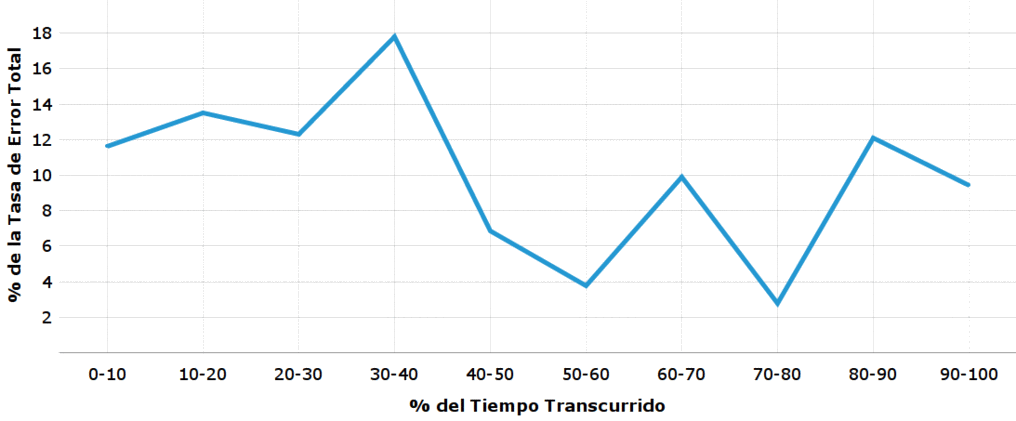
\includegraphics[width=0.8\linewidth]{./graphics/error_tiempo.png}
\caption{Distribuci\'on del error humano por etapas de la sesi\'on.}
\label{figure:gerror-tiempo}
\end{figure}
\end{frame}

\begin{frame}{Encuesta (1)}
\begin{table}[H] 
\centering
\footnotesize
\begin{tabular}{|r|r|r|r|r|}
\hline
    Sujeto & Palabras & Comandos & Entrenamiento & Interfaz por Voz \\
    \hline
    1 & 6 & 7 & 6 & 7 \\
    2 & 6 & 7 & 7 & 7 \\
    3 & 7 & 7 & 7 & 7 \\
    4 & 6 & 6 & 4 & 5 \\
    5 & 7 & 7 & 7 & 4 \\
    6 & 6 & 6 & 5 & 5 \\
    7 & 7 & 7 & 7 & 5 \\
    8 & 6 & 7 & 6 & 7  \\
    9 & 6 & 7 & 7 & 5  \\
    10 & 5 & 6 & 6 & 6  \\
    11 & 6 & 6 & 6 & 7  \\
    12 & 6 & 6 & 7 & 5  \\
\hline
\end{tabular}
\caption{Resumen de la encuesta realizada.}
\label{sec:tabla-encuesta}
\end{table}

\end{frame}


\begin{frame}{Encuesta (2)}
\begin{figure}[ht]
\centering
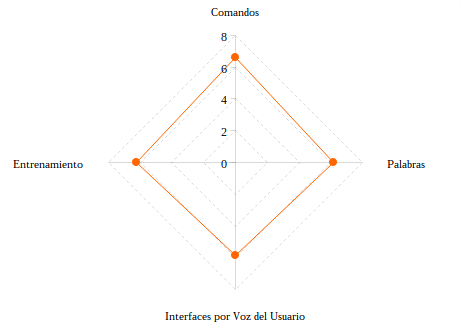
\includegraphics[width=0.6\linewidth]{./graphics/kiviat0.png}
\caption{Gr\'afico radial resumen de la encuesta realizada.}
\label{figure:kiviat-encuesta1}
\end{figure}
\end{frame}

\begin{frame}{Encuesta (3)}

\begin{table}[H] 
\centering
\footnotesize
\begin{tabular}{|r|r|r|r|r|}
\hline
    Sujeto &  Palabras & Comandos & Entrenamiento & Interfaz por Voz \\
    \hline
1 &  0 & 1 & 0 & 1\\
2 &  0 & 1 & 1 & 1\\
3 &  - & - & - & -\\
4 &  1 & 1 & 0 & 0,5\\
5 &  1 & 1 & 1 & 0\\
6 &  1 & 1 & 0 & 0\\
7 &  1 & 1 & 1 & 0\\
8 &  0 & 1 & 0 & 1\\
9 &  0,5 & 1 & 1 & 0\\
10 & 0 & 1 & 1 & 1\\
11 & 0 & 0 & 0 & 1\\
12 & 0,5 & 0,5 & 1 & 0\\
\hline
\end{tabular}
\caption{Resumen de la encuesta realizada. Valores reescalados.}
\label{sec:tabla-encuesta-normalizada}
\end{table}
\end{frame}

\begin{frame}{Encuesta (4)}
\begin{figure}[ht]
\centering
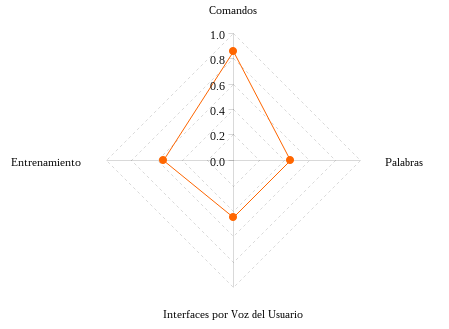
\includegraphics[width=0.6\linewidth]{./graphics/kiviat.png}
\caption{Gr\'afico radial resumen de la encuesta realizada. Valores reescalados.}
\label{figure:kiviat-encuesta2}
\end{figure}

\end{frame}
